\documentclass[12pt]{amsart}
\usepackage{geometry}                % See geometry.pdf to learn the layout options. There are lots.
\geometry{letterpaper}                   % ... or a4paper or a5paper or ... 
%\geometry{landscape}                % Activate for for rotated page geometry
%\usepackage[parfill]{parskip}    % Activate to begin paragraphs with an empty line rather than an indent
\usepackage{graphicx}
\usepackage{amssymb}
\usepackage[all]{xy}
\usepackage{epstopdf}
\usepackage{geometry}
\geometry{legalpaper, portrait, margin=1in}

\DeclareGraphicsRule{.tif}{png}{.png}{`convert #1 `dirname #1`/`basename #1 .tif`.png}


% these packages make it easy to include figures in the text. 
\usepackage{float}
\restylefloat{figure}

\newcommand{\lt}{\left}
\newcommand{\rt}{\right}
\newcommand{\la}{\lt\langle}
\newcommand{\ra}{\rt\rangle}
\newcommand{\ip}[1]{\la #1 \ra}
\newcommand{\T}{^{\mathsf{T}}}
\newcommand{\R}{\mathbb{R}}
\newcommand{\E}{\mathbb{E}}
\newcommand{\cX}{\mathcal{X}}
\newcommand{\cC}{\mathcal{C}}
\newcommand{\cF}{\mathcal{F}}

\DeclareMathOperator*{\argmin}{argmin}

% Path for the graphics
\graphicspath{ {../R/Graphs/} {../Report/Luke_final_project_latex/}}

\begin{document}
{\bf \Large AMATH 521 Final Project}\\
\begin{center}
{\bf \Large Topic: Sector Outperformance Analysis}\\
\end{center}
\vskip 16pt \noindent
{\textbf{Contributors}: }
\vskip 8pt \noindent
1.) Luke Lee\\
2.) Wipada Wannasiwaporn

\vskip 8pt \noindent
{\textbf{Summary}: }
\vskip 8pt \noindent
The goal of this project was to build a model that predicts the sectors that tend to outperform the market return using logistic regression with different penalties and try out different models for comparison. In order to confine our scope of the project, we decided to focus on the two largest sector in S\&P500, Technology and Financial. 

%==============================================
\begin{center}
	\line(1,0){450}
	\vskip 8pt \noindent
	{\bf Technology Sector}
\end{center}
\vskip 8pt \noindent
{\textbf{Data}: }
\vskip 8pt \noindent
Our independent variables are basically the monthly macro economics data retrieved from FRED(https://fred.stlouisfed.org/). Some examples of these data are unemployment 
rate, FED funds rate, CPI, SP500 monthly return etc. We also added some sector related data such as Telecommunication export to possibly add prediction power for a specific sector as well. We convert these raw data into a return space using monthly simple return for an Index-like data and use percentage conversion for a probability data and rate data. Here are some samples of our data.\\

% Table generated by Excel2LaTeX from sheet 'tech_raw_data'
\begin{table}[htbp]
	\centering
	\caption{Data Example}
	\begin{tabular}{rrrrrrr}
		\multicolumn{1}{l}{Date} & \multicolumn{1}{l}{IYW return} & \multicolumn{1}{l}{GDP} & \multicolumn{1}{l}{CSUSHPINSA} & \multicolumn{1}{l}{DGS10} & \multicolumn{1}{l}{TEDRATE} & \multicolumn{1}{l}{FEDFUNDS} \\
		10/31/2000 & -0.080775444 & 0.011088 & 0.005507 & 0.0577 & 0.0057 & 0.0651 \\
		11/30/2000 & -0.234329233 & 0.011088 & 0.005198 & 0.0548 & 0.0068 & 0.0651 \\
		12/31/2000 & -0.087222647 & 0.011088 & 0.004617 & 0.0512 & 0.0067 & 0.064 \\
		01/31/2001 & 0.172170997 & 0.003422 & 0.003953 & 0.0519 & 0.0056 & 0.0598 \\
	\end{tabular}%
	\label{tab:addlabel}%
\end{table}%
\vskip 8pt \noindent

For Technology Sector, we use BlackRock's ETF(IYW) that tracks the Technology sector performance using Dow Jones as a benchmark. Overall, the returns of Technology sector moves strongly correlated with the return of S\&P500 as seen in the high correlation value.
\begin{center}
	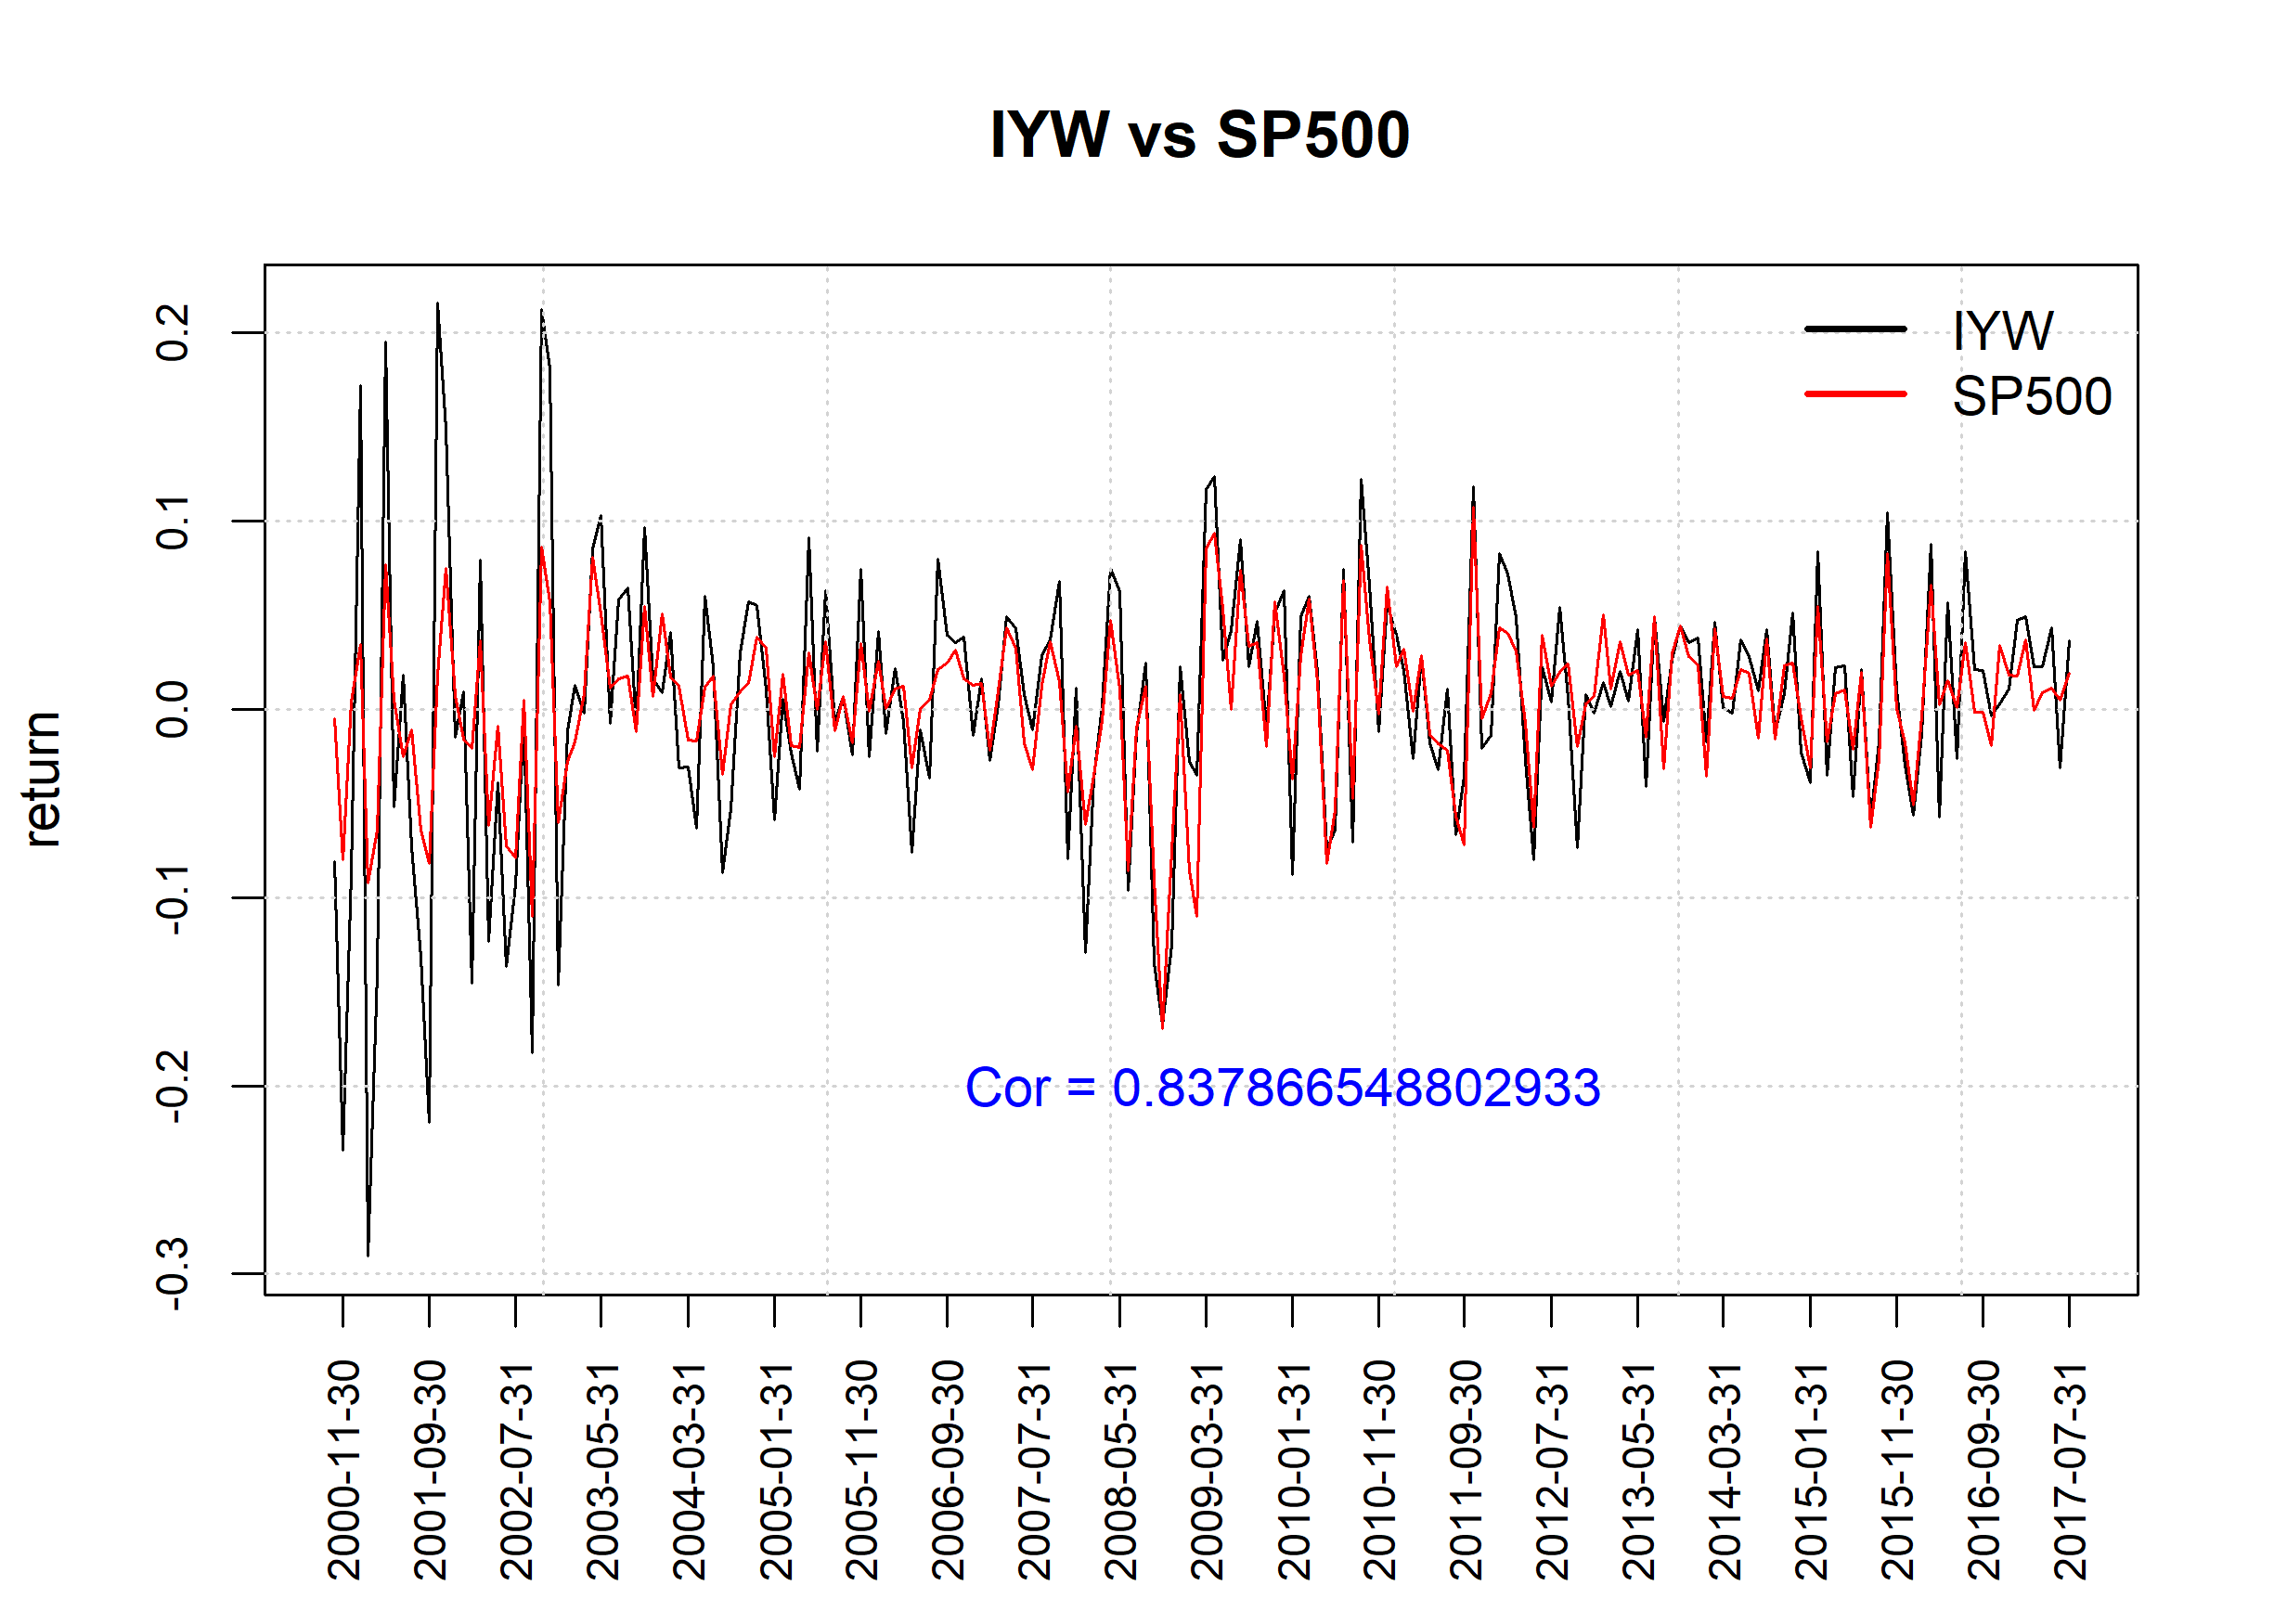
\includegraphics[scale=0.7]{IYW_vs_SP500}
\end{center}


%==============================================

\newpage

\vskip 8pt \noindent
{\textbf{Methods \& Algorithms}: }
\vskip 8pt \noindent

\textbf{i)} Linear Regression\\
We first want to make sure that our data can explain the data well, so doing linear regression is one way of doing sanity check on our data. By using our whole data set, it turns out that the explained variance($R^{2}$) is quite high for this data set, so we know our independent variables can somehow explain our dependent variable. 
\[ \mathbf{r} \in \R^{T}, \mathbf{F} \in \R^{T \times n}, \mathbf{x} \in \R^{n}
\]
\begin{align*}
\mathbf{r} \sim F_{1}x_{1} + F_{2}x_{2} + ... + F_{n}x_{n}
\end{align*}

where $\mathbf{r}$ represents our sector return(IYW - dependent variable) and $\mathbf{x}$ represents our economics data(independent variables).\\
The results of this linear regression shown a high coefficient of determination $R^{2}$.

\begin{figure}[htb]
	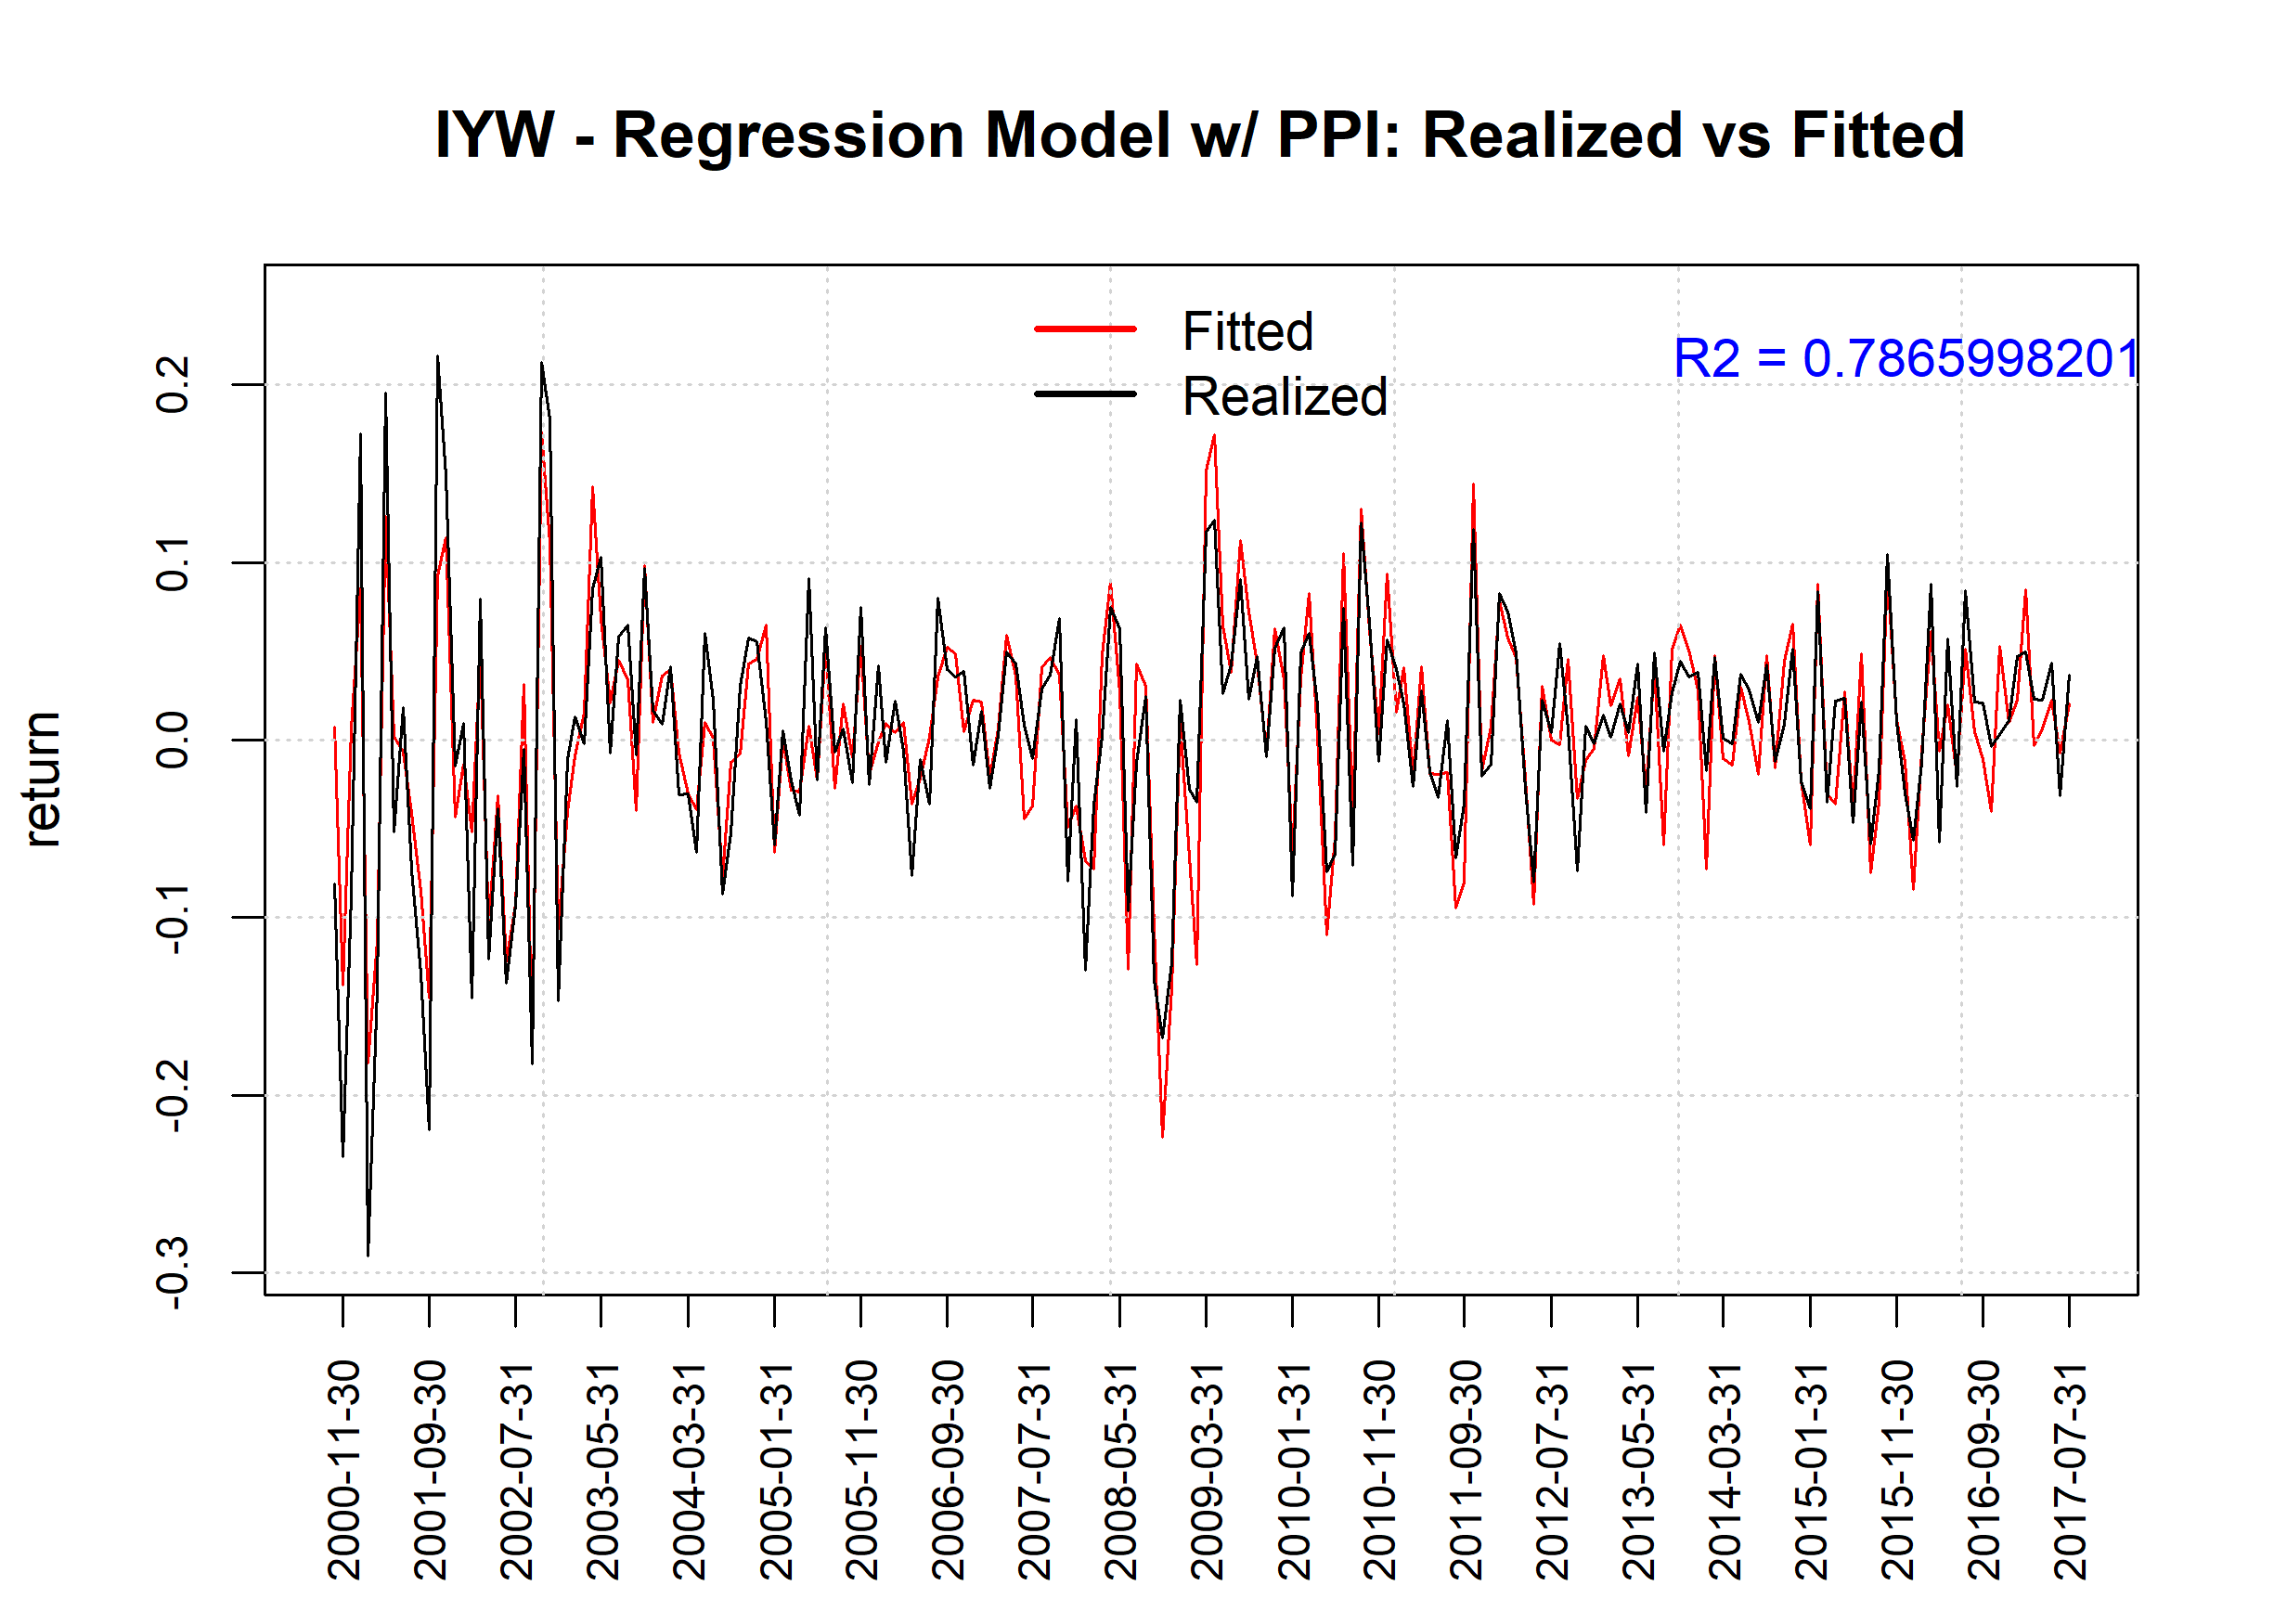
\includegraphics[scale=0.8]{IYW_linear_reg_withPPI}
\end{figure}

After doing some sanity check, we try to predict whether IYW will beat the market in the next period by assuming we know the exact values of our independent variables. We use the combination of rolling windows of 5, 6, 7, ..., 10 years of training samples to predict the next 1, 2, 3, ..., 6 months return. \\
After we get our predicted return, we check whether this return is greater than the market and use this as a boolean result of our linear regression. Using this boolean output, we can assess our outperformance accuracy by using
 
\begin{align*}
Accuracy = \frac{Numbers\ of\ correct\ predictions}{Numbers\ of\ total\ predictions}.
\end{align*}

Using accuracy as our selected criterion, we ran different combination of windows size and as a result, using 7 years of training data and 2 months of prediction period will give us the highest accuracy for linear regression method.

\newpage

The plots below show the result of prediction using 7 years training data to predict the next 2 months value.
\begin{figure}[htb]
	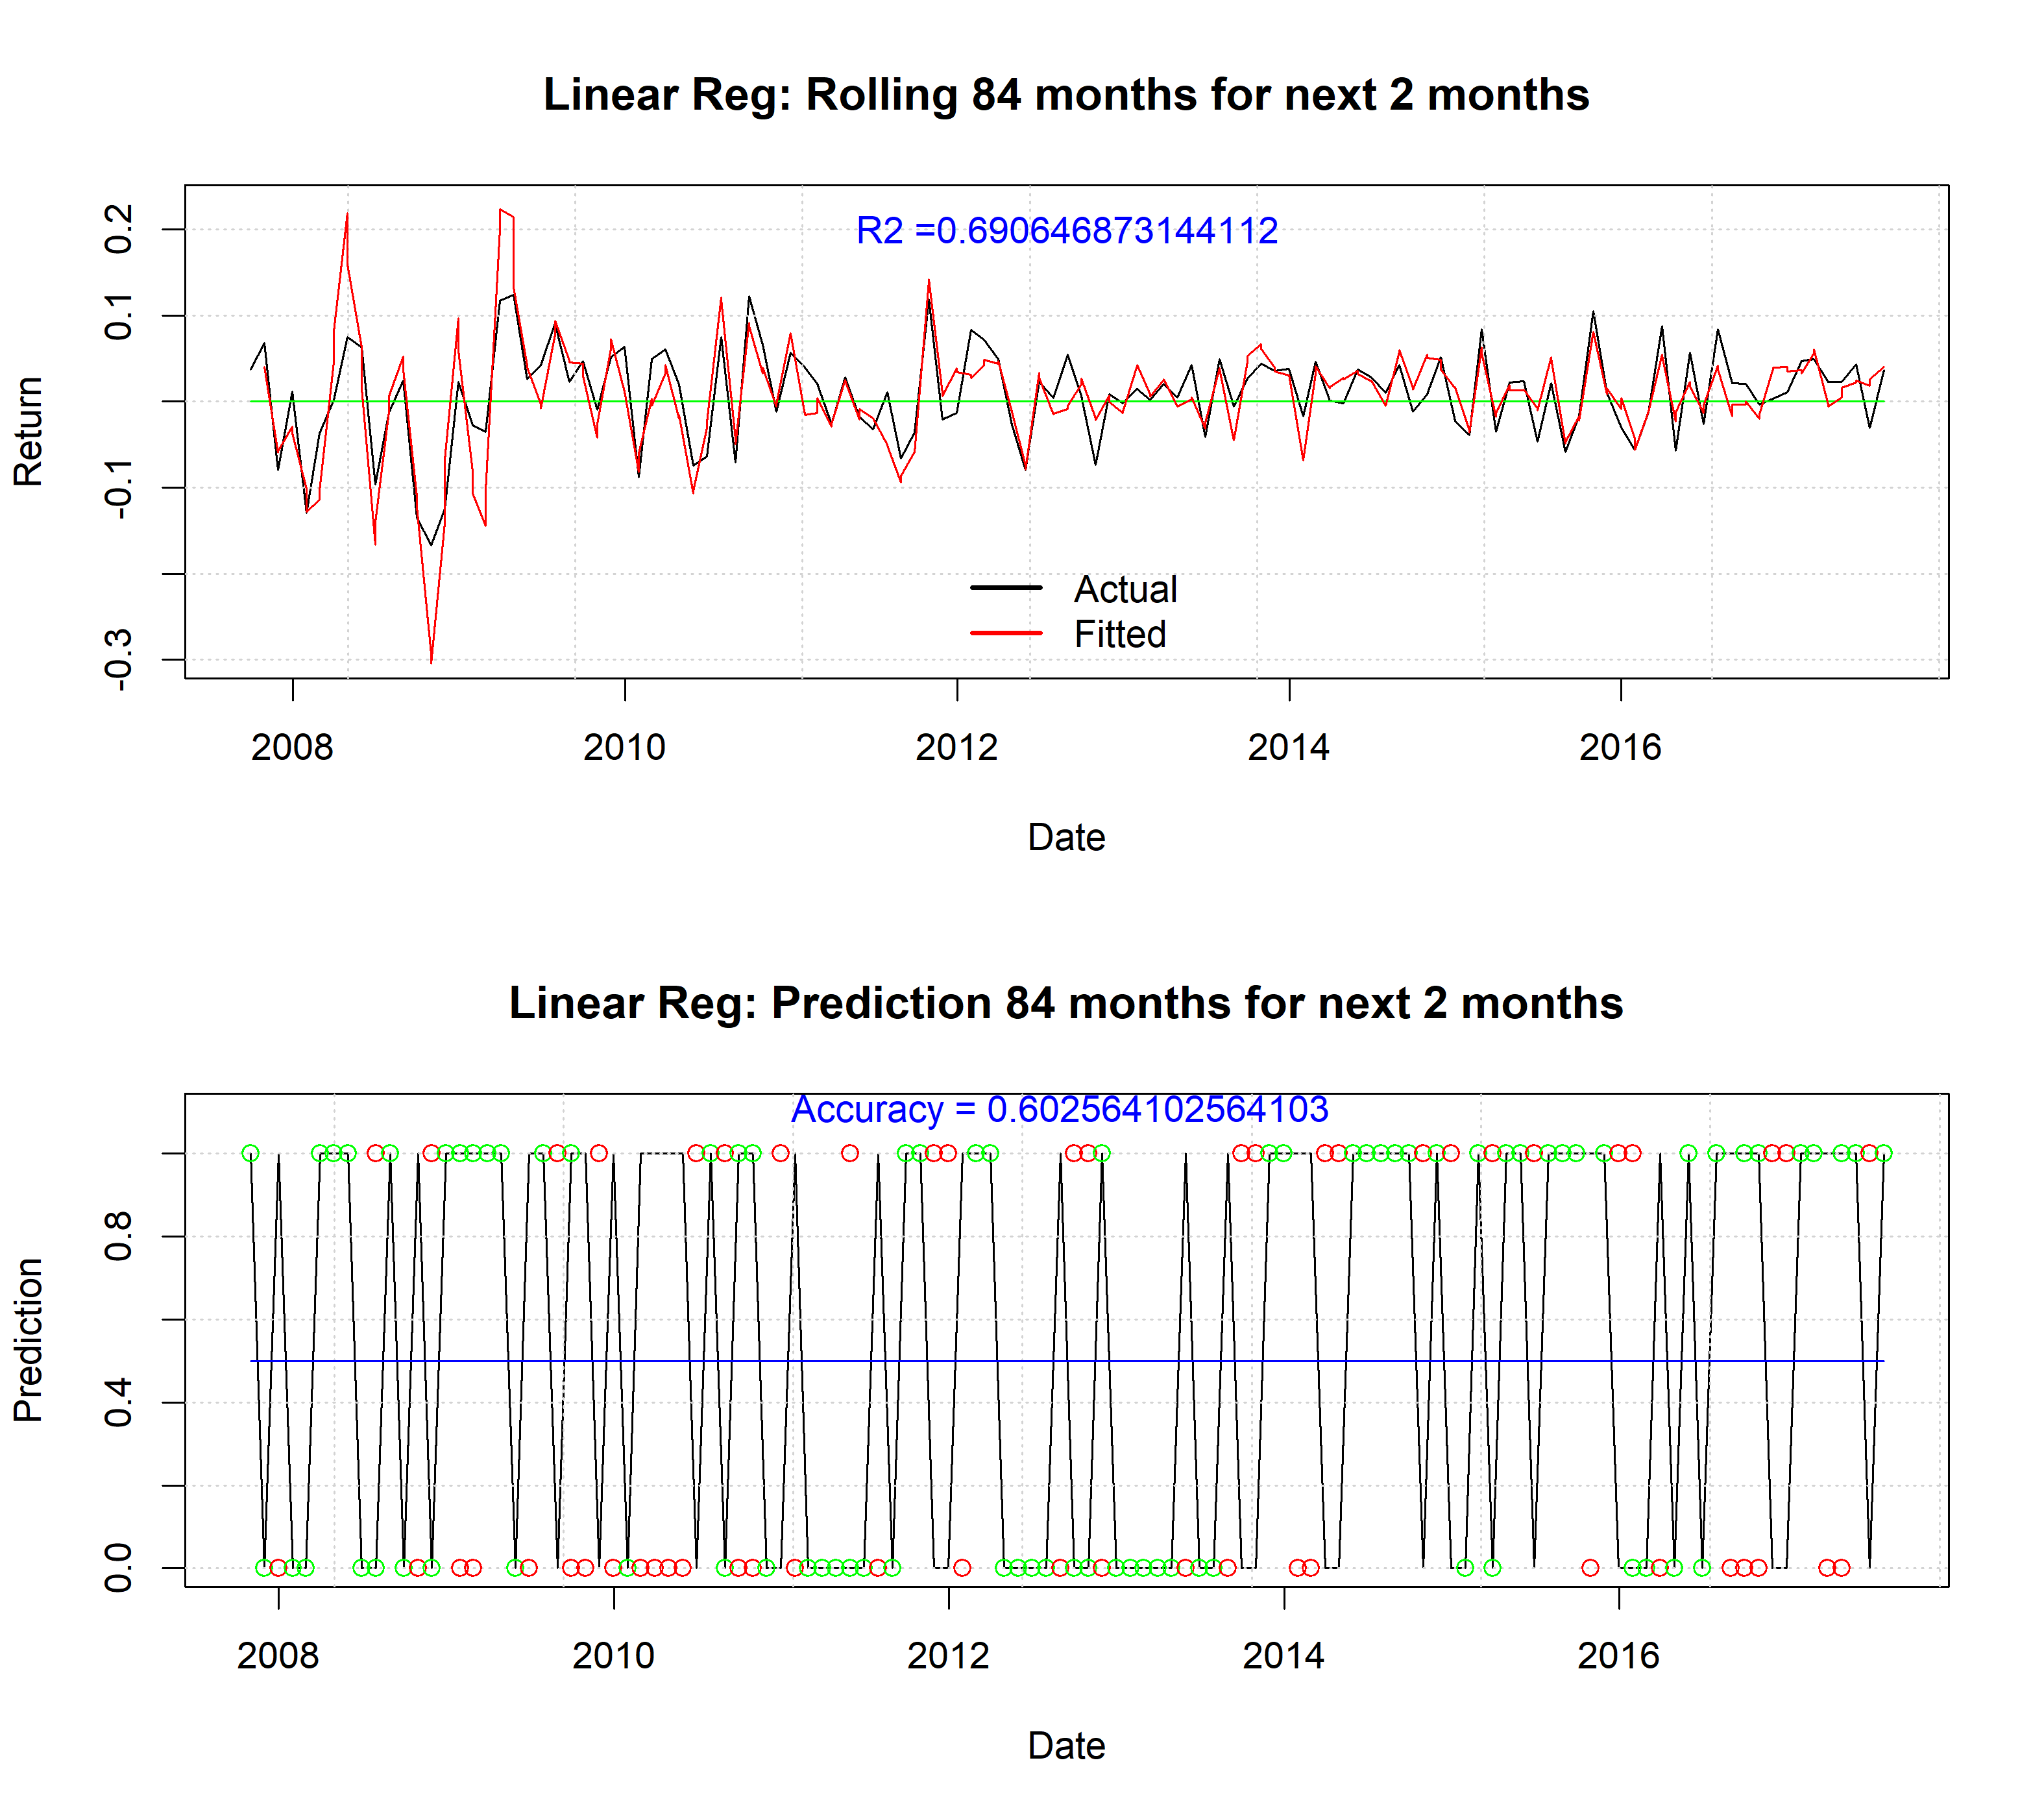
\includegraphics[scale=0.75]{IYW_linear_reg_rolling}
	\caption{Linear Regression\label{overflow}}
\end{figure}

\newpage

\textbf{ii)} Linear Regression with Elastic Net\\

The plots below show the result of prediction using 9 years training data to predict the next 1 month value.
\begin{figure}[htb]
	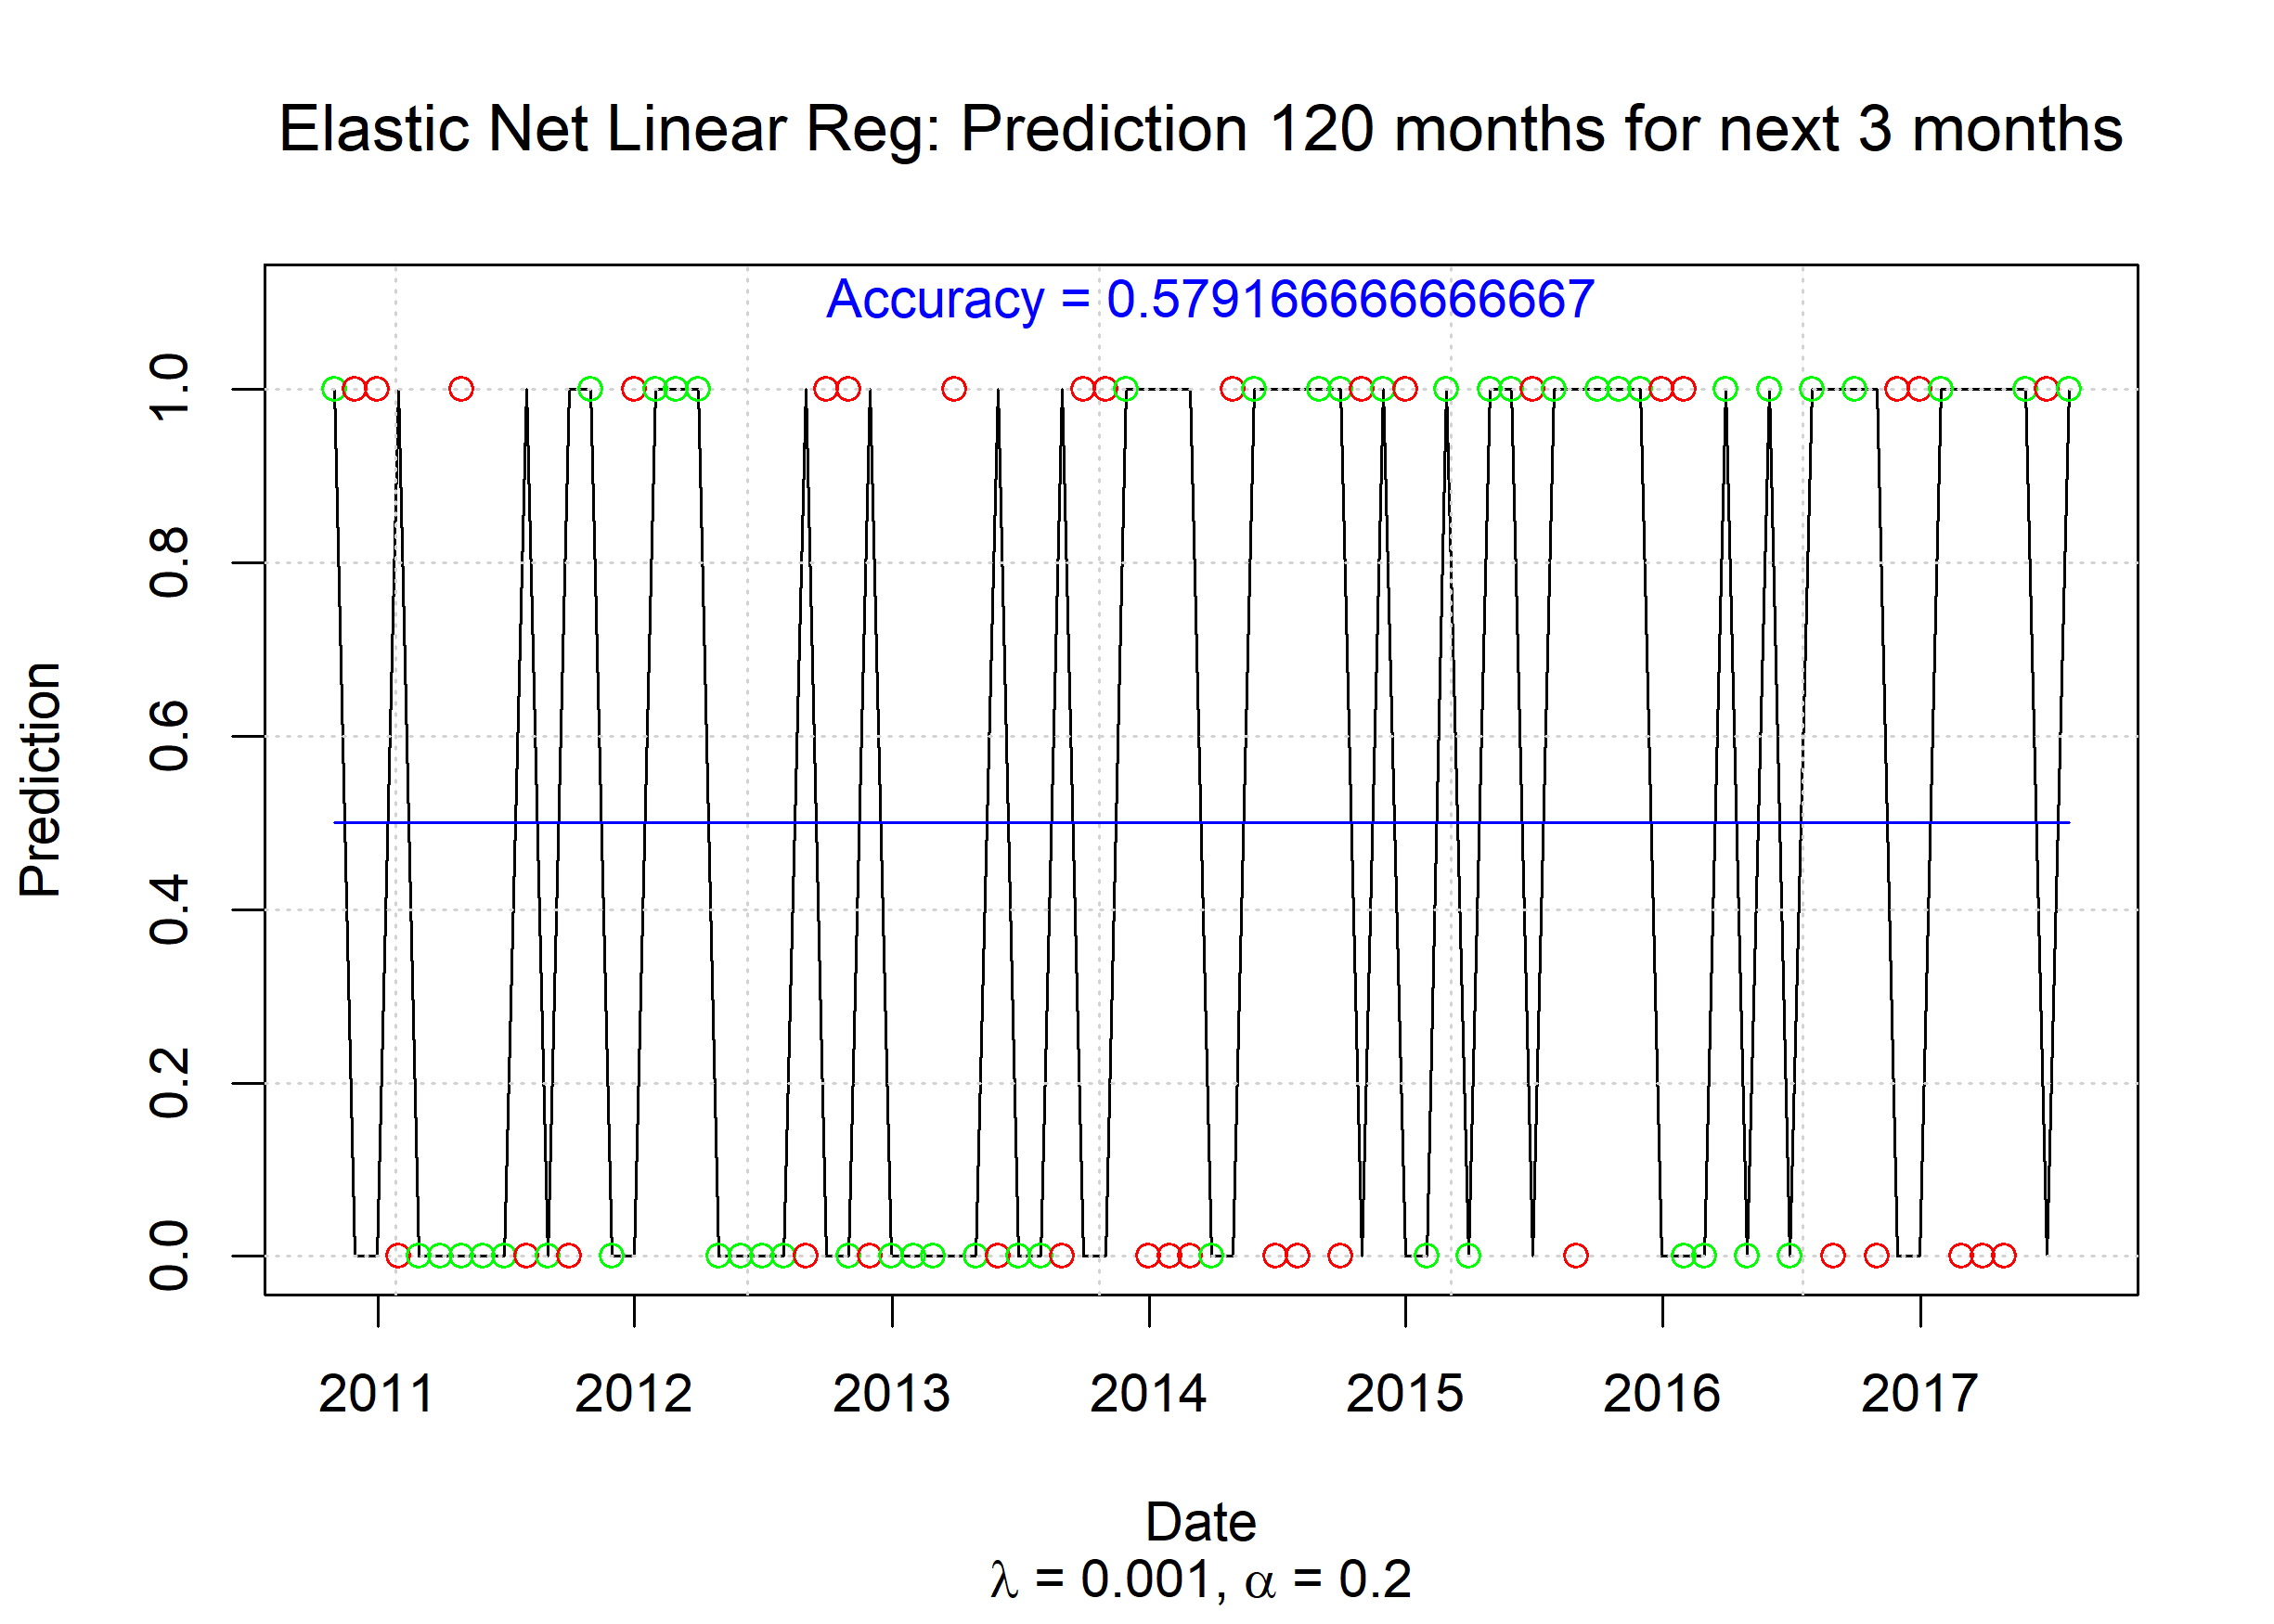
\includegraphics[scale=0.75]{IYW_linear_elastic_rolling}
	\caption{Linear Regression with Elastic Net\label{overflow}}
\end{figure}

\newpage

\textbf{iii)} Logistic Regression\\
The plots below show the result of prediction using 10 years training data to predict the next 2 months value.
\begin{figure}[htb]
	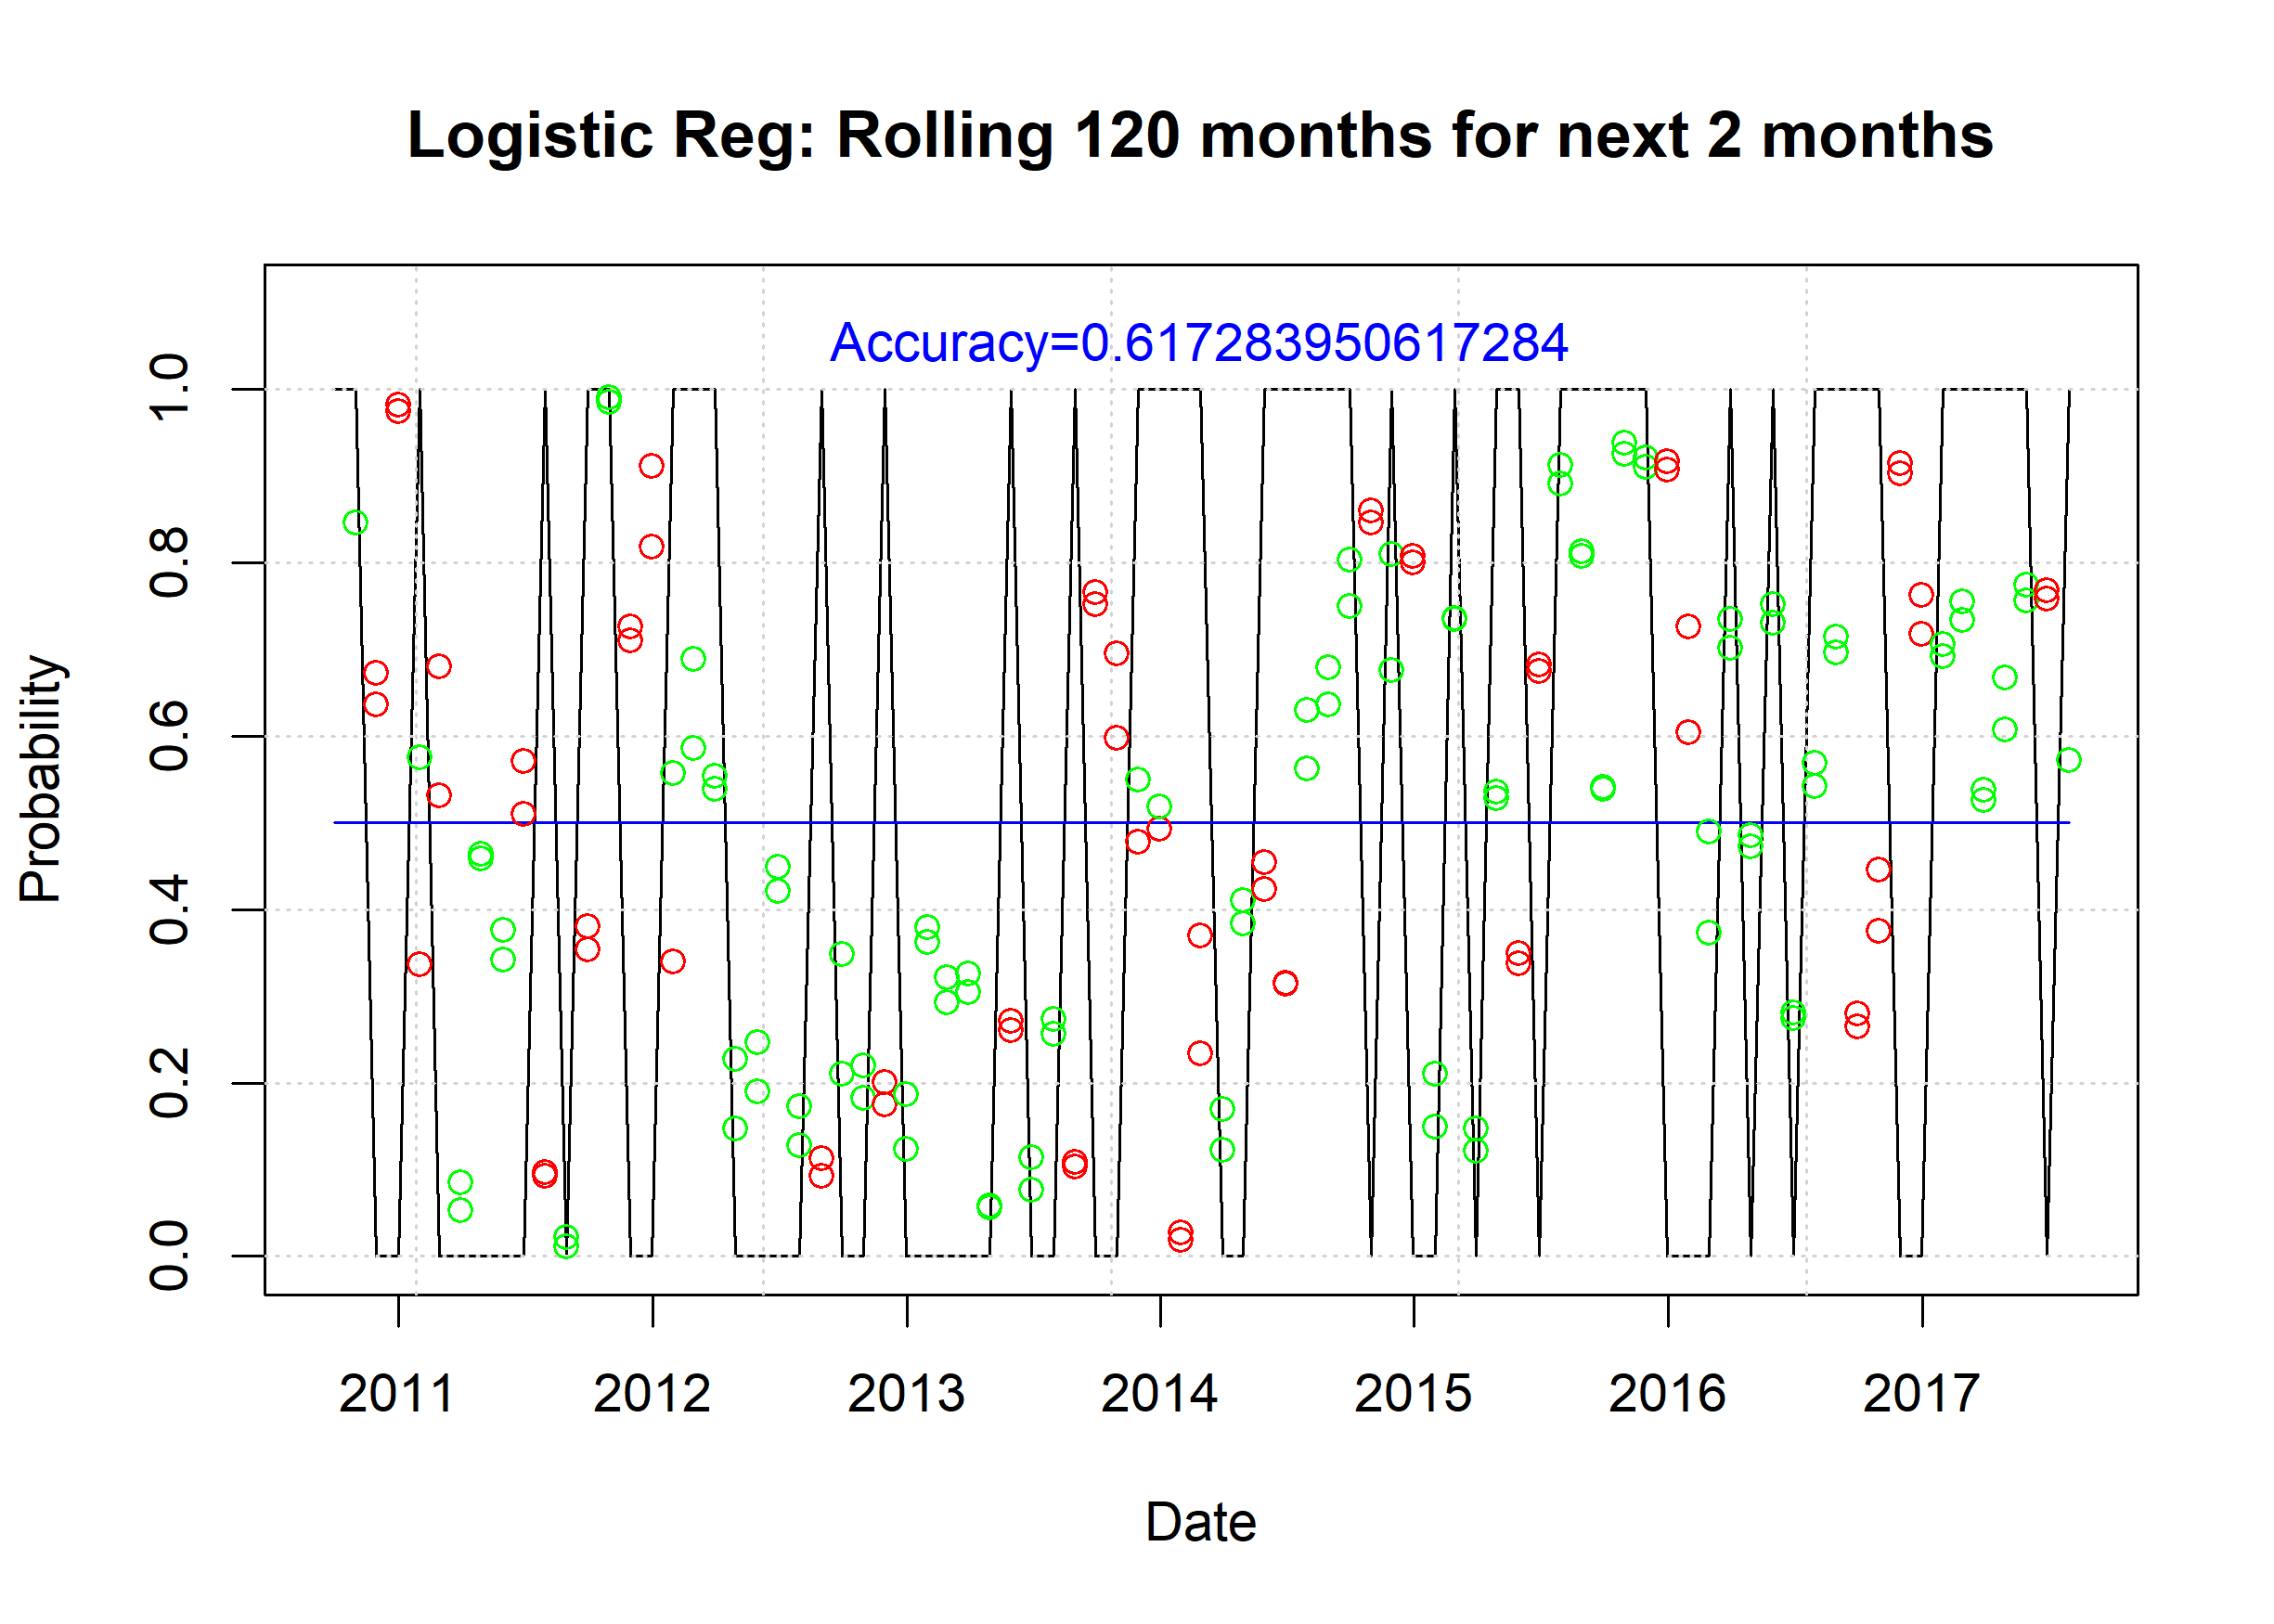
\includegraphics[scale=0.9]{IYW_logistic_reg_rolling}
	\caption{A simple caption \label{overflow}}
\end{figure}


\textbf{iv)} Logistic Regression with Elastic Net\\

\begin{figure}[htb]
	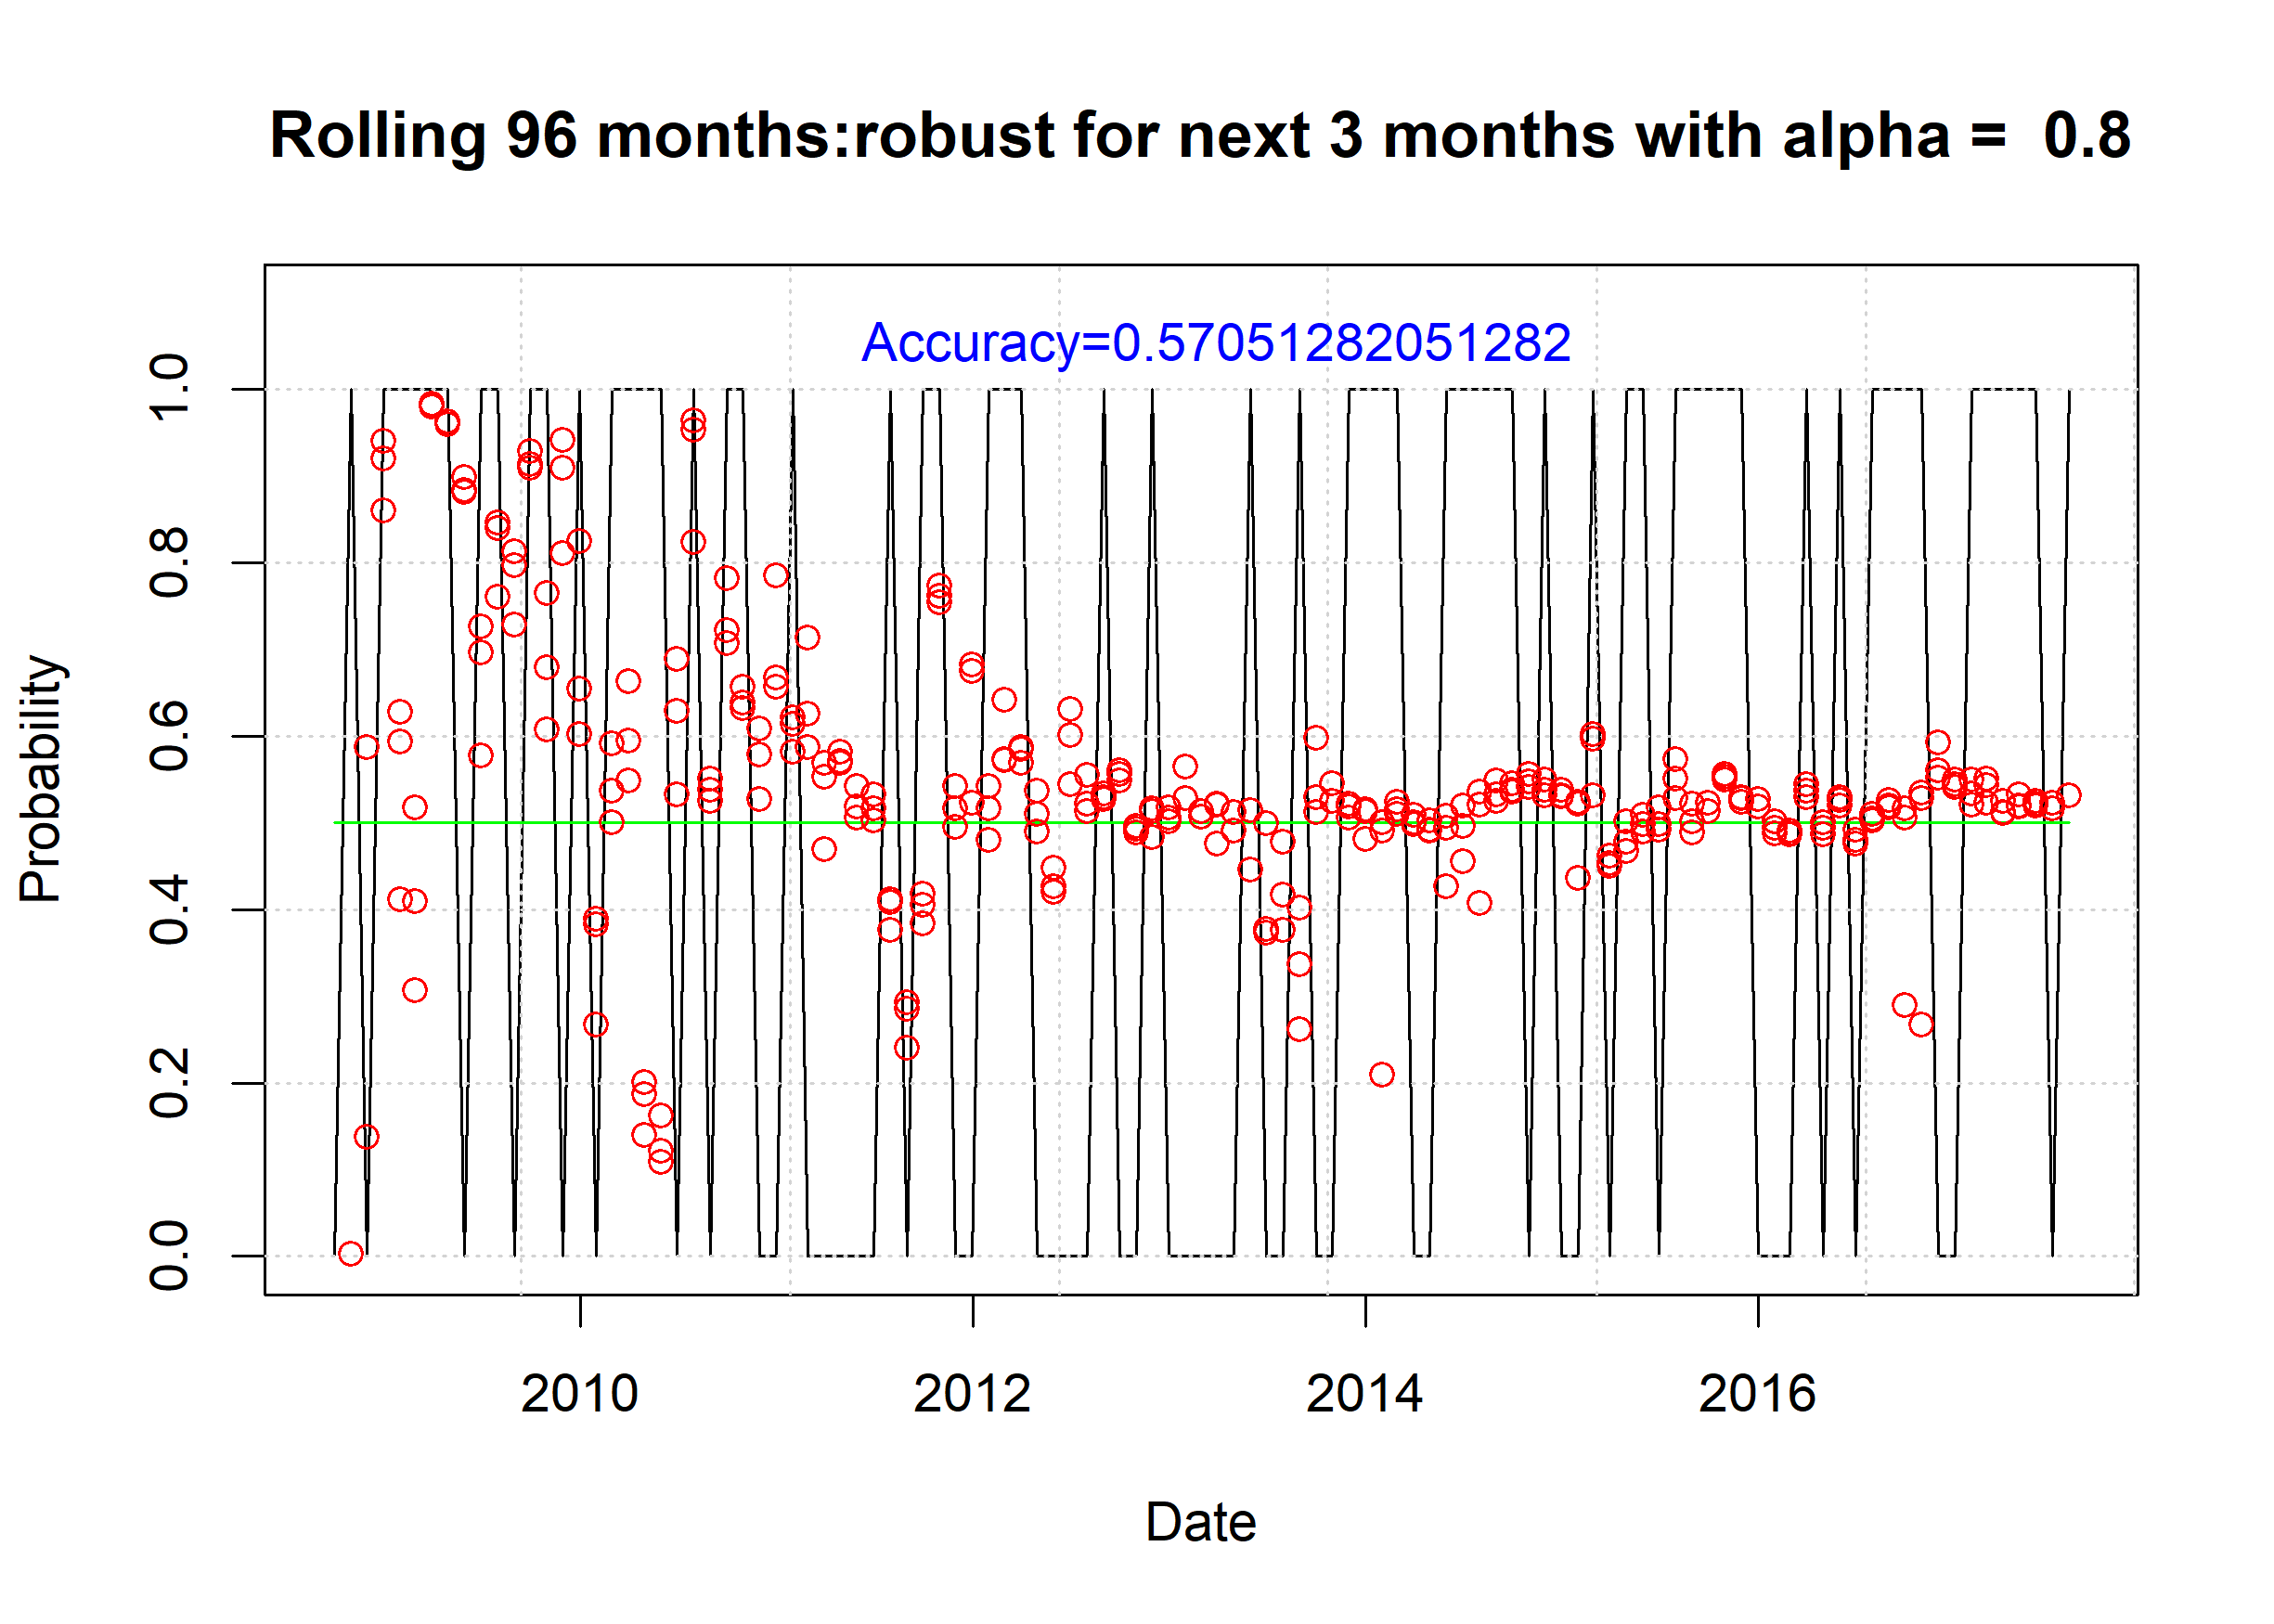
\includegraphics[scale=0.9]{IYW_logistic_elastic_rolling}
\end{figure}

\newpage

\textbf{v)} Support Vector Machine\\

\begin{figure}[htb]
	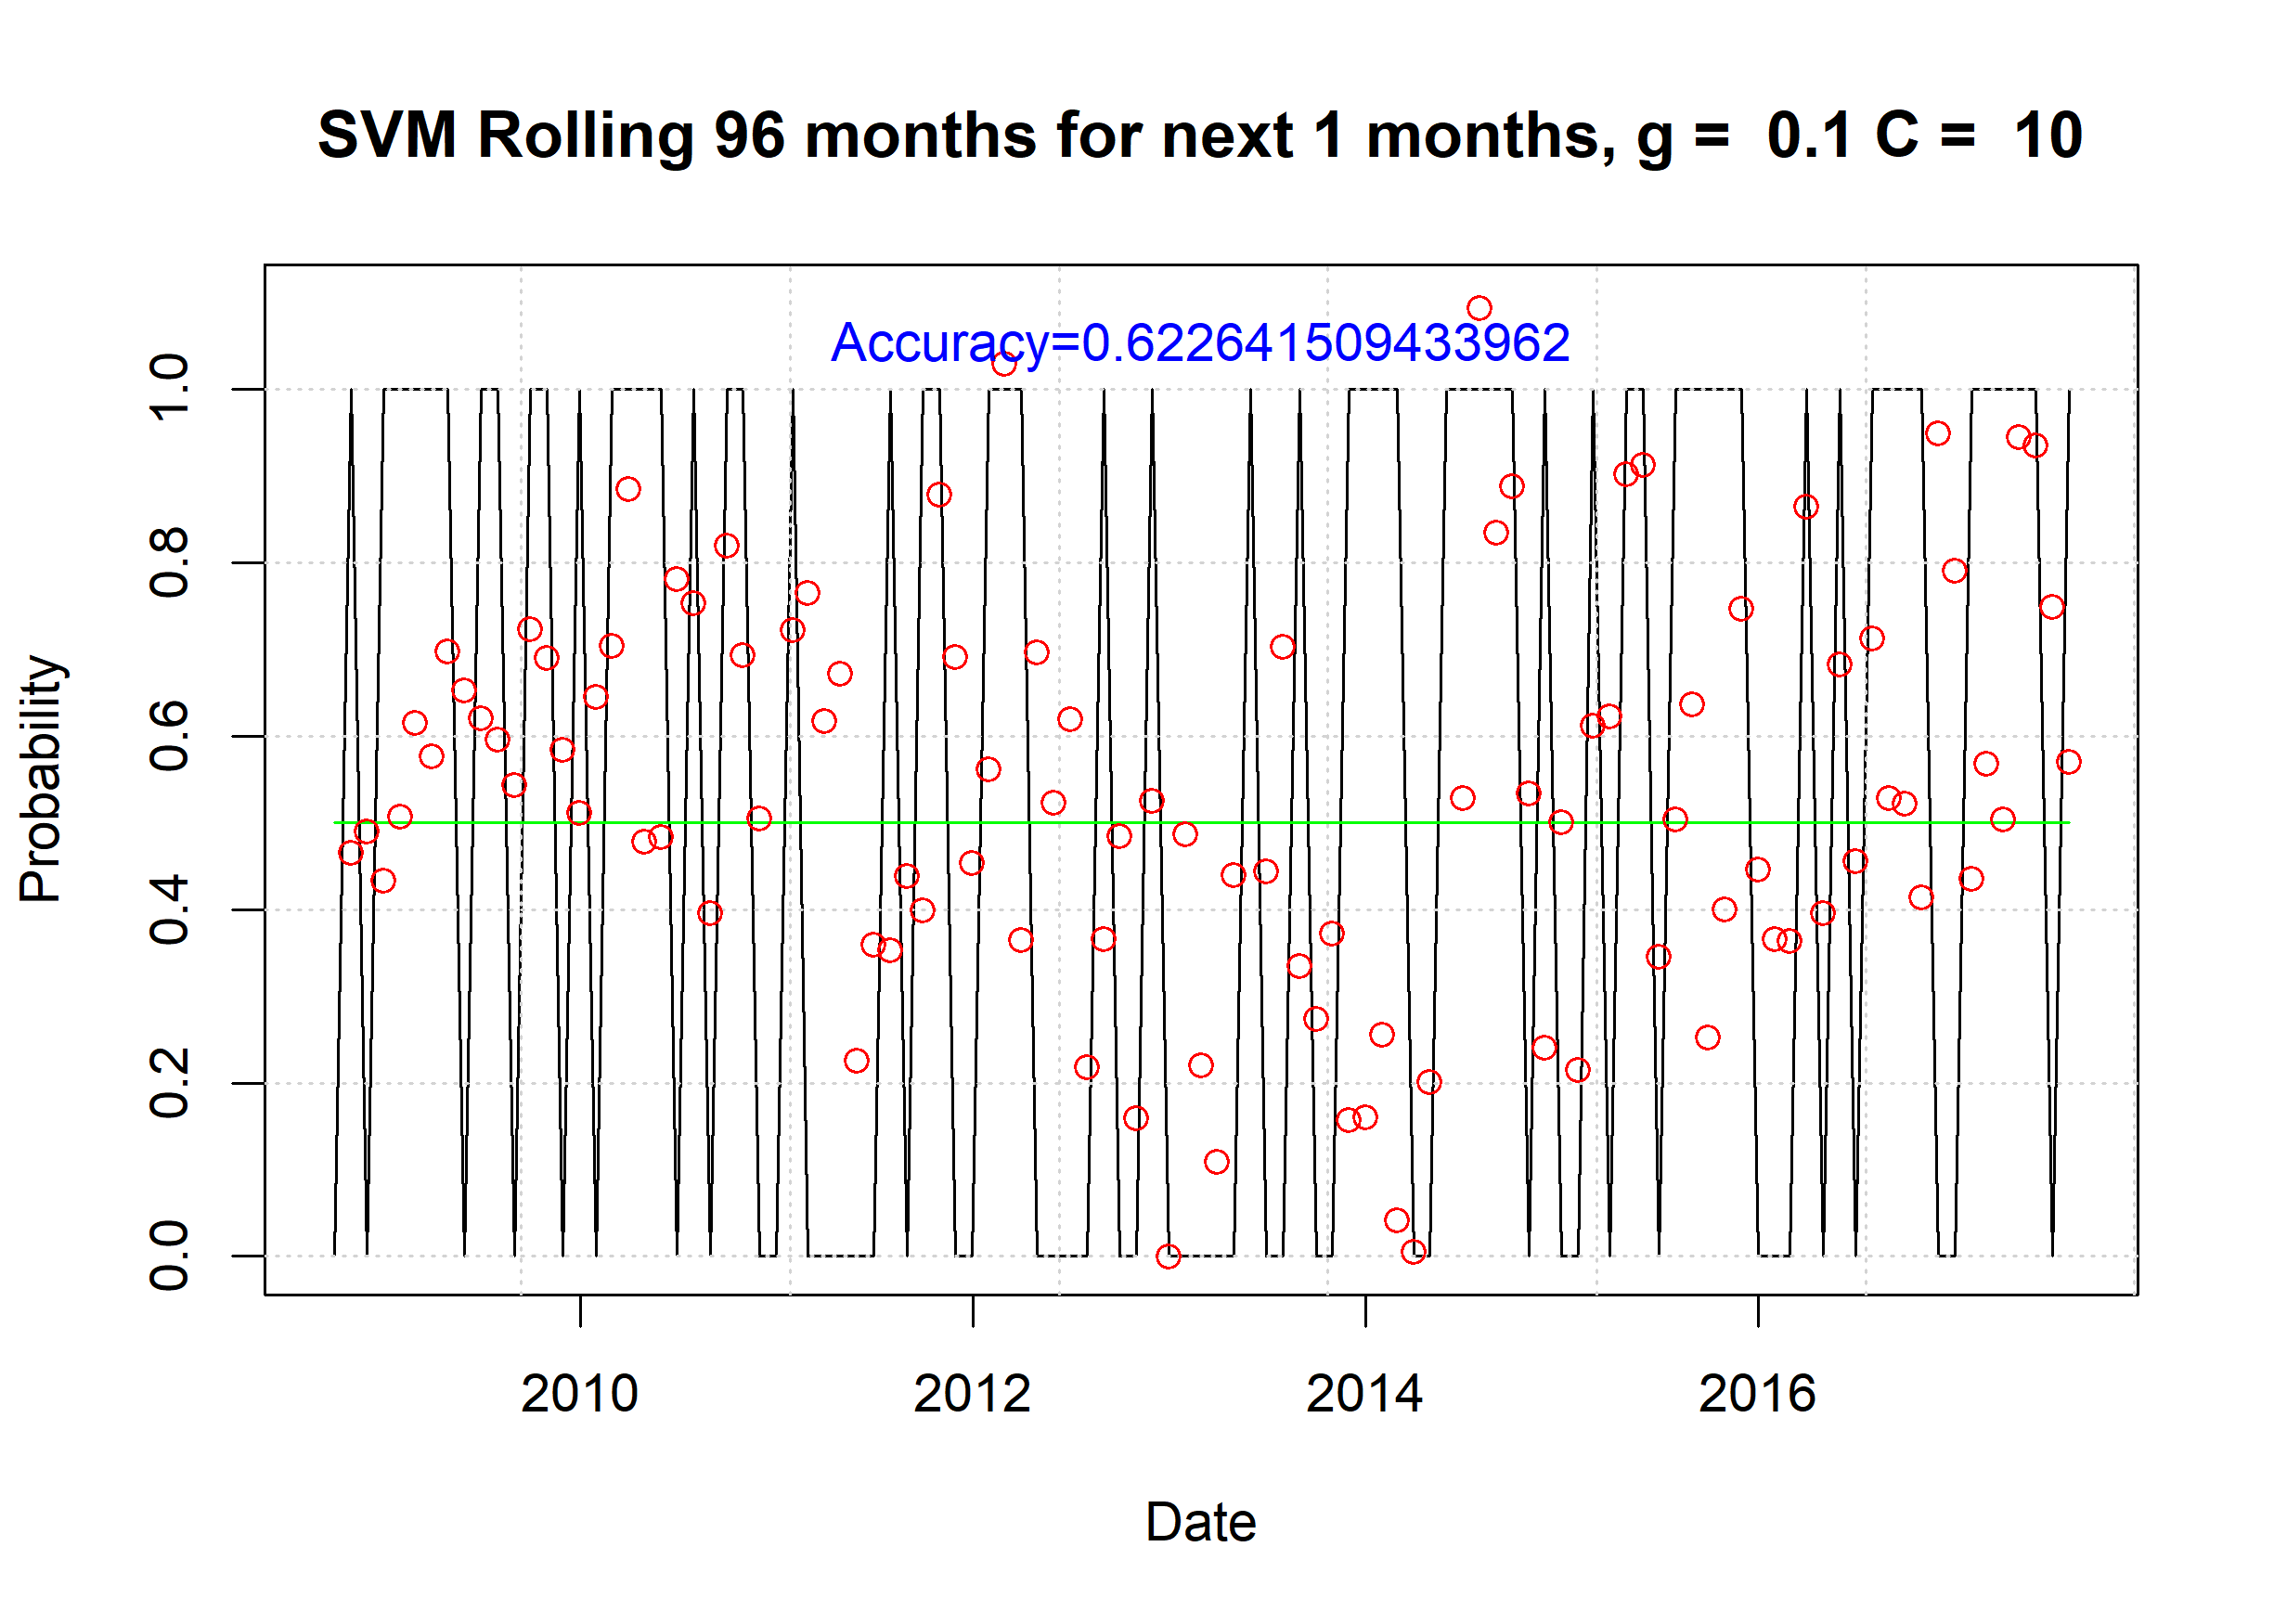
\includegraphics[scale=0.9]{IYW_SVM_rolling_penalize}
\end{figure}

gfjSGGJneklfniiqngienrhrbreqng

\newpage

%==============================================
\begin{center}
	\line(1,0){450}
	\vskip 8pt \noindent
	{\bf Financial Sector}
\end{center}

\vskip 8pt \noindent
{\textbf{Linear regression}: }
\vskip 8pt \noindent
Data selection  
\\
To verify that the data chosen for the financial sector(IYF iShare) we fit a linear regression and see if our underlying data can explain the sector returns. As shown in the figure below the selected data have a high $R^2$ value of $81.5 \%$
\begin{figure}[htb]
	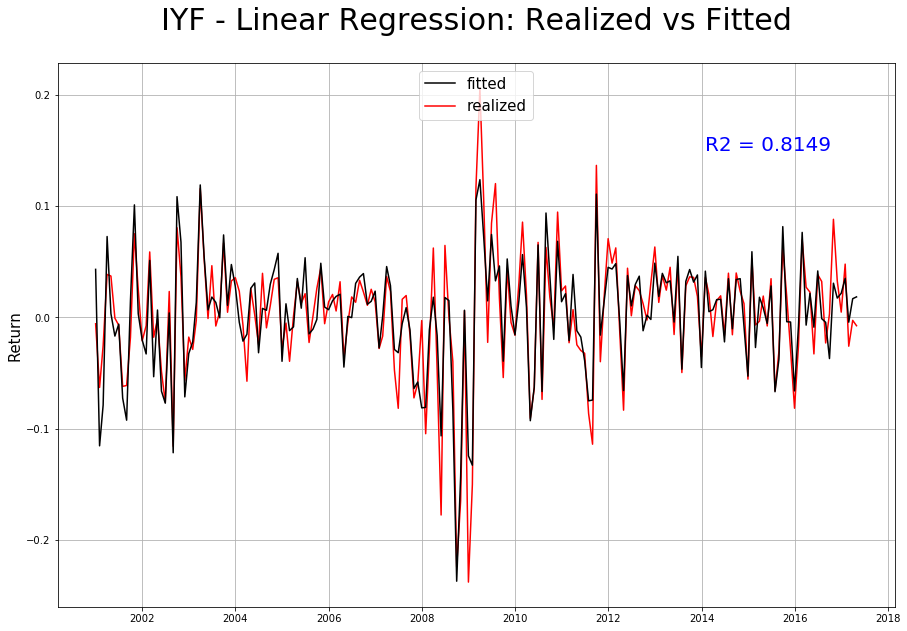
\includegraphics[scale=0.5]{linear_regression_additional_data.png}
\end{figure}
\\
Now that I am satisfied with the data selection, we can move on to testing out more complicated methods that could help us predict this sector out-preforming the benchmark. We calculated our binary predictor variable by taking the excess return of our sector and assigned 1 when it was positive and 0 otherwise.
\\
\section*{Logistic regression}
As mentioned before we are applying a robust method where we use past n years of data to predict certain months ahead and applying this on a rolling basis. In addition to these two parameters, we need to select the penalty type (l1 or l2) and the penalty value($\lambda$). After trying numerous combinations of these parameter's the optimal parameters selected were 5 year looking window, forecasting 3 months ahead, penalty of l2, with lambda of 3.4. 
\begin{figure}[htb]
	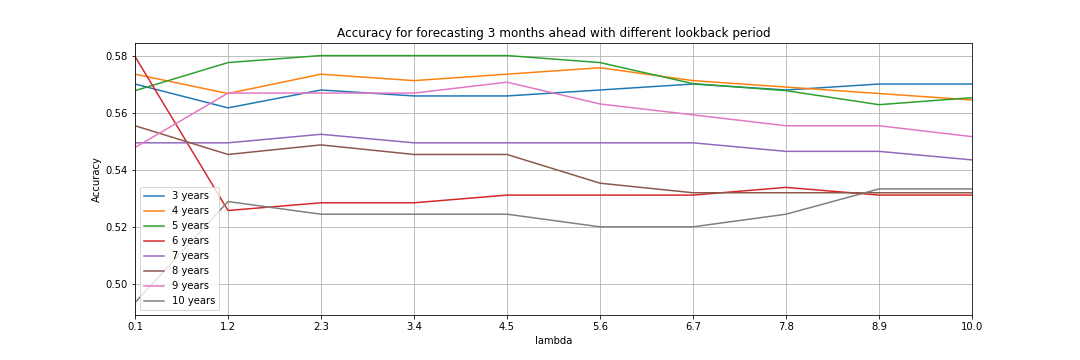
\includegraphics[scale=0.45]{logistic_acf_3month_result.png}
\end{figure}

Here is a comparison of predicted probability against the realized values.
\begin{figure}[htb]
	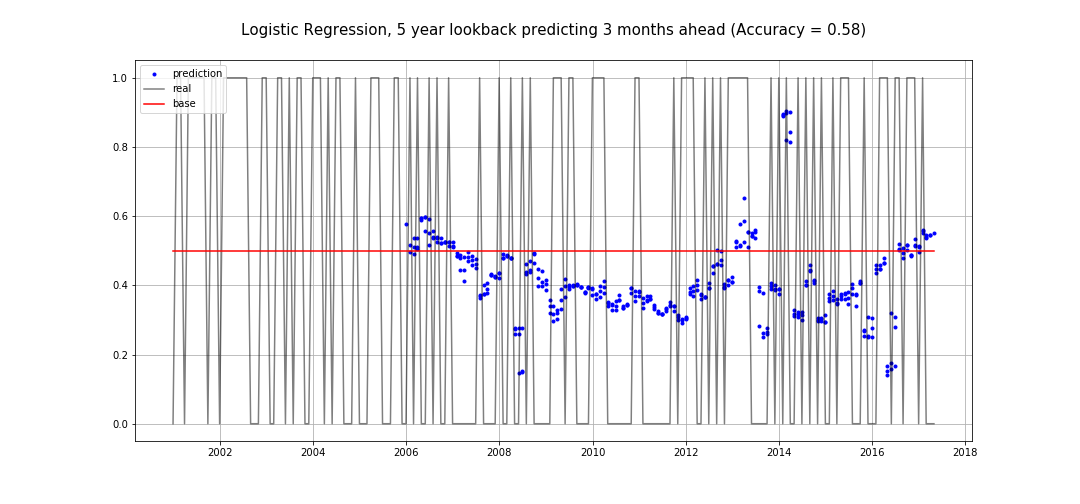
\includegraphics[scale=0.5]{Logistic_regression_5year_3months_result.png}
\end{figure}
The results were not as good as we have hoped for and partly because the probabilities we predict does not seem to be sparse. 

\section*{Elastic Net}
Another method we considered was Elastic Net. Elastic Net's objective function is an extension of linear regression it adds two additional terms, a L1 norm and a L2 norm.
\begin{align*}
\min_{w} \frac{1}{2n}  ||y - Xw||^2_2+\alpha \cdot \text{l1\_ratio} \cdot ||w||_1 + \frac{1}{2} \cdot \alpha \cdot (1 - \text{l1\_ratio}) \cdot ||w||^2_2
\end{align*}

As seen in the objective function, there are two parameters to choose from. $\alpha$ is the penalty parameter and L1\_ratio chooses the ratio of the L1 and L2 penalties.  

Unfortunately, the optimal parameter chosen for this model seem to be basically linear regression. The combination with the highest accuracy was when $\alpha$, the penalty parameter, was zero. This simply equates to linear regression.
\begin{figure}[htb]
	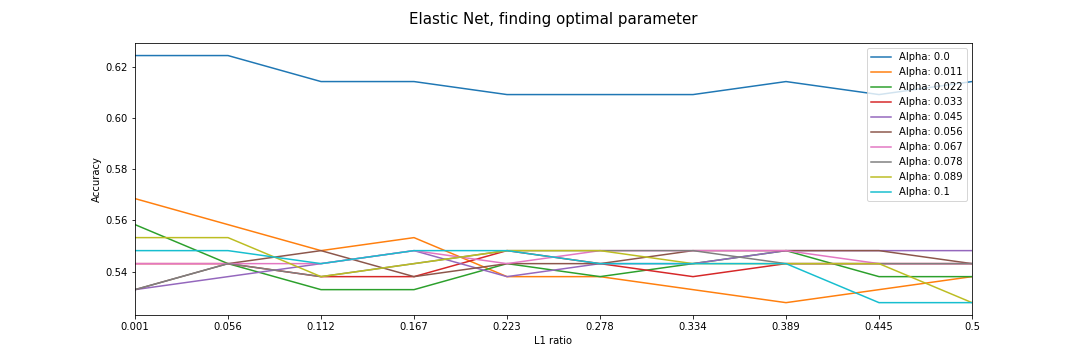
\includegraphics[scale=0.5]{Elastic_regression_cant_beat_linear_reg.png}
\end{figure}

\section*{Back to Linear regression}
Applying the same rolling basis method, linear regression still outperforms the other methods with $70.72\%$ accuracy. Interestingly, linear regression seem to do better with shorter training set data. The optimal parameter for this model was looking back 3 years to predict 3 months return ahead.

\begin{figure}[htb]
	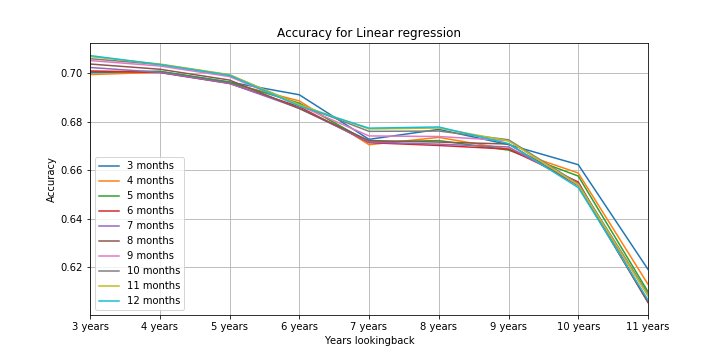
\includegraphics[scale=0.7]{Linear_regression_param.png}
\end{figure}


%==============================================

\newpage

\vskip 8pt \noindent
{\textbf{Summary \& Comments}: }
\vskip 8pt \noindent



\end{document}  
